\documentclass{standalone}
\usepackage{tikz}
\usepackage{xcolor}

\begin{document}

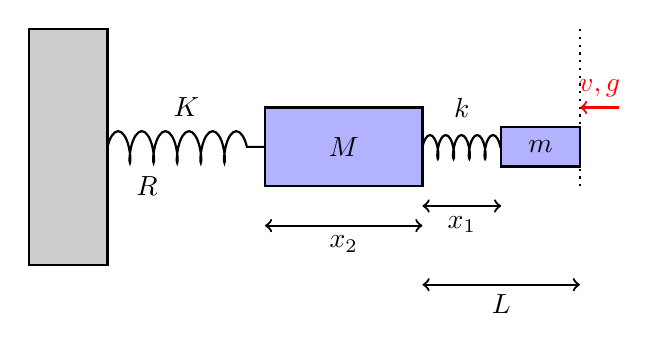
\begin{tikzpicture}[thick, scale=1]

% Colors
\definecolor{masscolor}{rgb}{0.7,0.7,1}

% Wall
\draw[fill=black!20] (-1, -0.5) rectangle (0, 2.5);

% Left spring
\draw[decoration={aspect=0.3, segment length=3mm, amplitude=2mm, coil}, decorate] (0,1) -- (2,1);

% Mass M
\filldraw[fill=masscolor] (2, 0.5) rectangle (4, 1.5);
\node at (3, 1) {$M$};

% Right spring
\draw[decoration={aspect=0.3, segment length=2mm, amplitude=1.5mm, coil}, decorate] (4,1) -- (5,1);

% Mass m
\filldraw[fill=masscolor] (5, 0.75) rectangle (6, 1.25);
\node at (5.5, 1) {$m$};

% Dashed lines and labels
\draw[dotted] (6, 0.5) -- (6, 2.5);
\draw[<->] (4, 0.25) -- node[below] {$x_1$} (5, 0.25);
\draw[<->] (2, 0) -- node[below] {$x_2$} (4, 0);

% L label
\draw[<->] (4, -0.75) -- node[below] {$L$} (6, -0.75);

% Forces
\draw[->, red, thick] (6.5, 1.5) -- ++(-0.5, 0);
\node[red, above] at (6.25, 1.5) {$v, g$};

% Labels for springs and wall
\node at (1, 1.5) {$K$};
\node at (4.5, 1.5) {$k$};
\node at (0.5, 0.5) {$R$};

\end{tikzpicture}

\end{document}